\documentclass[10pt,journal,compsoc]{IEEEtran}

\usepackage{amsmath,amssymb,amsfonts}
\usepackage{algorithmic}
\usepackage{graphicx}
\usepackage{textcomp}
\usepackage{xcolor}
\usepackage{booktabs}
\usepackage{cite}
\usepackage{url}
\usepackage{hyperref}
\usepackage{microtype}

\hypersetup{
    colorlinks=true,
    linkcolor=blue,
    citecolor=blue,
    urlcolor=blue
}

\begin{document}

\title{Reliability-Conditioned Prediction of Herb--Drug Interactions with Evidence Lineage Analysis, Citation Echo Detection, and Calibrated Abstention}

\author{Aditi~Sharma,~\IEEEmembership{Student Member,~IEEE}
\thanks{Manuscript received October 2026. The author is with the Department of Computer Science and Engineering, specializing in Biomedical Data Mining and Machine Learning.}
}

\markboth{IEEE Transactions on Neural Networks and Learning Systems / Bioinformatics, Under Review}%
{Sharma: Reliability-Conditioned Prediction of Herb--Drug Interactions}

\IEEEtitleabstractindextext{%
\begin{abstract}
Concurrent administration of botanical supplements and prescription pharmaceuticals is increasingly prevalent in modern healthcare, yet predicting herb--drug interactions (HDIs) remains a critical bioinformatics challenge. Unlike synthetic drug--drug interactions (DDIs) involving single active pharmaceutical ingredients, botanicals are complex multi-constituent mixtures whose scientific literature is corrupted by citation echo chambers (where dozens of secondary reviews reiterate an isolated index report), experimental context heterogeneity (in vitro vs. mammalian vs. human trials), and uncalibrated scientific contradictions. Here, we present a reliability-conditioned herb--drug interaction prediction framework that unifies: (1) evidence lineage directed acyclic graph (DAG) construction with connected-component echo attenuation ($\alpha = 0.15$); (2) multi-factor pharmacokinetic context compatibility scoring grounded in regulatory guidelines; (3) a heterogeneous Biological Graph Attention Network (GAT) over phase I/II human enzymes gated dynamically with BiomedBERT contextual embeddings; and (4) a validation-calibrated tri-state decision engine with epistemic uncertainty abstention. Evaluated on an auditable benchmark of 141 verified publications spanning 18 herbs and 40 prescription medications across 123 independent study clusters under strict study-disjoint partitioning (90 train, 25 validation, 26 test records), our architecture achieves 0.9762 ROC-AUC [95\% CI: 0.910, 1.000], 0.9707 PR-AUC, 0.9167 F1-score, and 92.31\% test accuracy (24/26 correct), providing absolute gains of +16.07 to +19.05 ROC-AUC points (+19.7\% to +24.2\% relative gain) over DeepDDI, KGNN, and CompGCN. Furthermore, calibrated abstention selectively identifies high-conflict trials, elevating diagnostic accuracy on non-conflicting queries to 96.00\% (24/25 correct).
\end{abstract}

\begin{IEEEkeywords}
Herb--Drug Interactions, Graph Attention Networks, Biomedical NLP, Evidence Lineage, Citation Echo Chambers, Uncertainty Calibration, Selective Classification.
\end{IEEEkeywords}}

\maketitle
\IEEEdisplaynontitleabstractindextext
\IEEEpeerreviewmaketitle

\section{Introduction}
\IEEEPARstart{C}{oncurrent} consumption of herbal supplements and conventional pharmaceutical therapies has surged worldwide. Over 35\% of adults in North America and Europe, and more than 70\% across Asia, report regular co-administration of botanicals alongside chronic medications~\cite{izzo2012interactions}. Unlike synthetic small molecules characterized by single, well-defined active pharmaceutical ingredients (APIs), botanical preparations (e.g., \textit{Hypericum perforatum} [St. John's wort], \textit{Ginkgo biloba}, \textit{Panax ginseng}, \textit{Curcuma longa}) comprise intricate phytochemical matrices consisting of dozens of pharmacologically active secondary metabolites~\cite{foti2012botanical}. These phytochemicals simultaneously modulate human phase I cytochrome P450 enzymes (e.g., CYP3A4, CYP2C9, CYP1A2), phase II glucuronosyltransferases, and membrane drug transporters (e.g., ABCB1/P-glycoprotein, OATP1B1/3).

Adverse herb--drug interactions (HDIs) induce severe clinical consequences, including organ transplant loss due to St. John's wort-induced clearing of cyclosporine and tacrolimus~\cite{ruschitzka1999stjohns}, fatal hemorrhages precipitated by Ginkgo biloba co-ingestion with warfarin, and cardiovascular collapse from ephedra-ephedrine interactions. Despite these clinical hazards, computational discovery of HDIs has lagged considerably behind drug--drug interaction (DDI) modeling. When conventional machine learning architectures developed for DDIs (e.g., DeepDDI~\cite{ryu2018deep}, KGNN~\cite{wang2019kgnn}, CompGCN~\cite{vashishth2020compgcn}) are adapted to herbal domains, they suffer from three structural vulnerabilities:

\begin{enumerate}
    \item \textbf{Citation Echo Chamber Inflation:} Scientific literature frequently suffers from citation cascades where an initial speculative case report is uncritically reiterated across dozens of secondary review articles, textbook chapters, and meta-commentaries. Traditional NLP and DDI models treat each text mention or publication as an independent observation, mistaking circular citation volume for genuine scientific consensus.
    \item \textbf{Experimental Context Mismatches:} An in vitro microsomal binding assay conducted at supraphysiological aglycone concentrations ($>100\,\mu\text{M}$) rarely translates to in vivo clinical bioavailability in humans, where gut microbiota deglycosylation, hepatic first-pass clearance, and plasma protein binding substantially attenuate systemic exposure. Existing algorithms aggregate in vitro and clinical reports indiscriminately.
    \item \textbf{Forced Binary Extrapolation under Scientific Contradiction:} Literature often contains contradictory clinical evidence (e.g., retrospective case reports attributing warfarin bleeding to cranberry juice vs. prospective randomized double-blind clinical trials demonstrating zero pharmacokinetic interaction). Standard binary classifiers force a hard interaction label, generating false positive alarms that drive clinical alert fatigue.
\end{enumerate}

To overcome these structural limitations, we formulate the \textbf{Reliability-Conditioned Herb--Drug Interaction Prediction System}, introducing an end-to-end framework that couples evidence lineage graphs, pharmacokinetic context weighting, heterogeneous biological graph attention, and validation-calibrated selective abstention.

\section{Related Work and Prior Art Analysis}

\begin{table*}[t]
\centering
\caption{Comparative Landscape and Prior Art Analysis}
\label{tab:prior_art}
\small
\begin{tabular}{lp{3.2cm}p{3.2cm}cc}
\toprule
\textbf{System / Prior Art} & \textbf{Technical Architecture} & \textbf{Data Modality} & \textbf{Lineage \& Echo Discounting?} & \textbf{Calibrated Abstention?} \\
\midrule
DeepDDI~\cite{ryu2018deep} & Deep MLP on molecular fingerprints & Synthetic chemical APIs & No (static labels) & No \\
KGNN~\cite{wang2019kgnn} & KG Convolution + Relation Attention & Topology over generic KGs & No (homogeneous edges) & No \\
CompGCN~\cite{vashishth2020compgcn} & Compositional multi-relational GCN & Relational graph triples & No & No \\
Patent CN115223731B~\cite{cn115223731b} & Dempster--Shafer theory + Dirichlet & Multi-sensor feature fusion & No (hard combination rules) & No (binary output) \\
HTINet2~\cite{htinet2024} & Herb-Target KG + GCN + BPR loss & Herb-Target bipartite graphs & No (static $p<0.05$ filter) & No \\
\textbf{Proposed System} & \textbf{Biological GAT + BiomedBERT + Reliability Gating} & \textbf{Audited Pharmacokinetic Graphs + Clinical Literature DAGs} & \textbf{Yes ($\mathcal{G}_L$ connected components, $\alpha=0.15$)} & \textbf{Yes (Epistemic MC Dropout + Conflict Abstention)} \\
\bottomrule
\end{tabular}
\end{table*}

Prior computational DDI architectures rely primarily on molecular graph convolutions, structural fingerprints, or knowledge graph link prediction. As detailed in Table~\ref{tab:prior_art}, models such as DeepDDI~\cite{ryu2018deep} operate on single chemical structures and cannot process multi-component botanical extracts. Graph-based formulations like KGNN~\cite{wang2019kgnn} and CompGCN~\cite{vashishth2020compgcn} treat interaction edges as static ground truth without verifying literature provenance. 

In patent literature, CN115223731B~\cite{cn115223731b} proposed fusing multi-source evidence using Dempster--Shafer (D-S) mathematical evidence theory and Dirichlet uncertainty modeling. However, CN115223731B assumes that input evidence channels are mutually independent; it does not construct citation lineage DAGs, lacks connected-component citation clustering, cannot detect circular echo cascades, and forces a closed-world decision without clinical abstention. Similarly, recent botanical models such as HTINet2~\cite{htinet2024} filter noisy literature via static heuristic $p$-value thresholds, discarding all dependency graphs and temporal ancestry.

Our framework is the first to directly model citation lineage graphs, attenuate circular echo amplification through connected components, and execute risk-calibrated clinical abstention.

\section{Proposed Methodology}

The architecture consists of four tightly integrated modules: (1) Evidence Lineage and Echo Attenuation; (2) Multi-Factor Pharmacokinetic Context Scoring; (3) Reliability-Conditioned Multimodal GNN Fusion; and (4) Validation-Calibrated Tri-State Abstention.

\subsection{Evidence Lineage and Echo Attenuation}
\textbf{Definition 1 (Citation Lineage Graph and Multi-Domain Edge Semantics):} For any herb--drug pair $(h, d)$, let $\mathcal{E}_{h,d} = \{e_1, e_2, \dots, e_N\}$ be the set of extracted literature evidence records indexed by verified DOIs and PMIDs. We construct a directed citation lineage graph $\mathcal{G}_L = (\mathcal{V}_L, \mathcal{E}_L)$, where each node $v_i \in \mathcal{V}_L$ corresponds to a scientific publication $s_i$. A directed edge $(v_i, v_j) \in \mathcal{E}_L$ indicates that study $s_i$ explicitly cites, reviews, or derives its clinical data from study $s_j$. Independent empirical investigations (clinical trials with distinct trial registrations or patient cohorts, animal studies with distinct protocols/groups, or in vitro studies from distinct laboratories/voucher specimens) are maintained as separate independent evidence roots, preventing independent trials from being collapsed merely because they are co-cited by a common review article.

\textbf{Definition 2 (Connected Component Echo Discounting):} Let $\mathcal{C}_1, \mathcal{C}_2, \dots, \mathcal{C}_K$ denote the weakly connected components of $\mathcal{G}_L$. In each component $\mathcal{C}_k$, the node with the earliest verified publication year is identified as the primary index study $s_{\text{primary}}^{(k)}$. All other nodes $s_j \in \mathcal{C}_k \setminus \{s_{\text{primary}}^{(k)}\}$ are classified as secondary echo publications. The effective independent cluster strength $S(\mathcal{C}_k)$ is computed as:
\begin{equation}
S(\mathcal{C}_k) = q(s_{\text{primary}}^{(k)}) + \sum_{s_j \in \mathcal{C}_k, j \neq \text{primary}} \alpha \cdot q(s_j)
\end{equation}
where $q(s) \in [0, 1]$ represents the study extraction quality score (incorporating trial design, sample size, and validation rigour), and $\alpha \in [0.05, 0.25]$ (nominal $\alpha = 0.15$) is the empirical echo attenuation discount factor.

\subsection{Multi-Factor Pharmacokinetic Context Compatibility}
Each evidence record $e_i$ is parameterized by an experimental context compatibility score $\mathcal{K}(e_i) \in [0, 1]$ reflecting regulatory principles from FDA botanical guidance and EMA DDI guidelines:
\begin{equation}
\mathcal{K}(e_i) = w_{\text{species}}(e_i) \cdot w_{\text{prep}}(e_i) \cdot w_{\text{route}}(e_i)
\end{equation}
where the contextual multipliers are:
\begin{align}
w_{\text{species}} &= \begin{cases} 1.00 & \text{Human clinical trial or PK study} \\ 0.65 & \text{In vivo mammalian (rodent, canine, porcine)} \\ 0.30 & \text{In vitro (microsomes, cell lines, recombinant)} \end{cases} \\
w_{\text{prep}} &= \begin{cases} 1.00 & \text{Standardized botanical extract (e.g., LI 160, EGb 761)} \\ 0.85 & \text{Crude whole-herb decoction / extract} \\ 0.70 & \text{Isolated pure single aglycone} \end{cases} \\
w_{\text{route}} &= \begin{cases} 1.00 & \text{Oral co-administration (canonical clinical route)} \\ 0.75 & \text{Parenteral (IV, IP)} \end{cases}
\end{align}

\subsection{Scientific Contradiction Index}
Let $S_{\text{pos}}$ and $S_{\text{neg}}$ denote the discounted cluster evidence strengths asserting interaction presence and interaction absence, respectively. The scientific contradiction index $C_{h,d} \in [0, 1]$ is formulated as:
\begin{equation}
C_{h,d} = \frac{2 \cdot \min(S_{\text{pos}}, S_{\text{neg}})}{S_{\text{pos}} + S_{\text{neg}} + \epsilon}
\end{equation}
where $\epsilon = 10^{-6}$. When evidence is strictly unipolar, $C_{h,d} = 0$. When equal evidence clusters report opposite conclusions, $C_{h,d} \to 1.0$.

\subsection{Dynamic Reliability Gating and Multimodal Fusion}
The composite evidence lineage vector $\mathbf{m}_{h,d} \in \mathbb{R}^{10}$ encompasses:
\begin{equation}
\mathbf{m}_{h,d} = \left[ S_{\text{pos}}, S_{\text{neg}}, N_{\text{primary}}, N_{\text{echo}}, \bar{\kappa}_{\text{context}}, C_{h,d}, \bar{q}, \Delta_{\text{time}}, N_{\text{raw,pos}}, N_{\text{raw,neg}} \right]
\end{equation}
The continuous scalar reliability coefficient $R_{h,d} \in [0, 1]$ is generated via a calibrated multi-layer perceptron:
\begin{equation}
R_{h,d} = \sigma\left(\mathbf{W}_2 \cdot \text{GELU}(\mathbf{W}_1 \mathbf{m}_{h,d} + \mathbf{b}_1) + b_2\right) \cdot \left(1 - \beta \cdot C_{h,d}\right)
\end{equation}
where $\beta \in [0.20, 0.60]$ (nominal $\beta = 0.40$) penalizes active scientific conflict.

\textbf{Pharmacodynamic Rationale for Reliability Gating:}
\begin{itemize}
    \item $\mathbf{z}_{\text{graph}}$ (Biological Mechanism Prior): Learned via a 2-layer Heterogeneous Biological GAT~\cite{velickovic2018gat} over human pharmacokinetic enzymes (CYP3A4, CYP2C9, CYP2C19, CYP2D6, CYP1A2, CYP2E1) and transporters (ABCB1, OATP1B1/3). This captures theoretical pharmacokinetic plausibility.
    \item $\mathbf{z}_{\text{contextual}}$ (In Vivo Clinical Text Representation): Extracted via frozen PubMedBERT/BiomedBERT~\cite{gu2021biomedbert} ($\mathbb{R}^{768}$) and projected onto the graph space using a training-exclusive SVD matrix $\mathbf{V}_{\text{train}}$. This captures empirical human trial observations.
\end{itemize}
In clinical pharmacology, verified in vivo human outcomes supersede in vitro theoretical plausibility. Hence, as literature reliability $R \to 1$, the model prioritizes $\mathbf{z}_{\text{contextual}}$. When literature is absent, speculative, or circular ($R \to 0$), the model smoothly retreats to the biological graph prior $\mathbf{z}_{\text{graph}}$:
\begin{equation}
\mathbf{z}_{\text{fused}} = (1 - R_{h,d}) \cdot \mathbf{z}_{\text{graph}} + R_{h,d} \cdot \mathbf{z}_{\text{contextual}}
\end{equation}

\subsection{Validation Temperature Scaling and Tri-State Abstention}
Raw link prediction logits $z$ are calibrated using validation-set temperature scaling~\cite{guo2017calibration} optimized strictly on the held-out validation split $\mathcal{D}_{\text{val}}$:
\begin{equation}
T^* = \arg\min_T -\sum_{(x, y) \in \mathcal{D}_{\text{val}}} \left[ y \log \sigma\left(\frac{z(x)}{T}\right) + (1-y) \log\left(1 - \sigma\left(\frac{z(x)}{T}\right)\right) \right]
\end{equation}
yielding calibrated posterior probability $\hat{p} = \sigma(z / T^*)$.

\textbf{Tri-State Clinical Decision Rule:} Let $u_{\text{epistemic}}$ be the predictive variance across $M=10$ Monte Carlo dropout passes~\cite{gal2016dropout} with rate $p_{\text{drop}} = 0.15$. The final classification $\hat{Y}(h, d)$ follows:
\begin{equation}
\hat{Y} = \begin{cases}
\text{ABSTAIN} & \text{if } u_{\text{epistemic}} > \tau_u \;\lor\; \left( C_{h,d} > \tau_c \;\land\; |\hat{p} - 0.5| < \tau_{\text{margin}} \right) \\
\text{INTERACTION} & \text{else if } \hat{p} \ge 0.50 \\
\text{NO INTERACTION} & \text{else if } \hat{p} < 0.50
\end{cases}
\end{equation}
with clinical safety parameters $\tau_u = 0.25$, $\tau_c = 0.50$, and $\tau_{\text{margin}} = 0.35$. When the Abstain state is triggered, the system routes the query to an asynchronous clinical review queue and displays an advisory flag rather than generating false-positive alarms or unsafe silence.

\section{Empirical Evaluation}

\subsection{Audited Real-World Benchmark}
The benchmark dataset consists of \textbf{141 peer-reviewed scientific publications} registered with 100\% verified PubMed PMIDs and DOIs across 18 botanicals and 40 prescription pharmaceuticals spanning oncology, cardiology, neurology, and transplantation, organized into \textbf{123 independent study clusters}. 

\textbf{Study-Disjoint Splitting Protocol:} Weakly connected citation components are indivisibly partitioned: 60\% train (90 records, 73 clusters), 20\% validation (25 records, 25 clusters), and 20\% test (26 records, 25 clusters). Zero citation ancestors or descendants appear across splits.

\subsection{Comparative Performance Against Baselines}
Table~\ref{tab:results} summarizes performance on the study-disjoint test partition of 26 records. Our proposed framework achieves an ROC-AUC of \textbf{0.9762 [95\% CI: 0.910, 1.000]} and an accuracy of \textbf{92.31\% (24/26 correct)}, providing absolute gains of +16.07 to +19.05 ROC-AUC points (+19.7\% to +24.2\% relative gain) over published baselines DeepDDI, KGNN, and CompGCN.

\begin{table*}[t]
\centering
\caption{Benchmark Evaluation on Study-Disjoint Test Splits (26 Records across 25 Clusters)}
\label{tab:results}
\small
\begin{tabular}{lcccccc}
\toprule
\textbf{Model Architecture} & \textbf{ROC-AUC (95\% CI)} & \textbf{PR-AUC} & \textbf{F1-Score} & \textbf{ECE} & \textbf{Brier Score} & \textbf{Accuracy} \\
\midrule
\textbf{Proposed Reliability-Conditioned} & \textbf{0.9762 [0.910, 1.000]} & \textbf{0.9707} & \textbf{0.9167} & \textbf{0.1650} & \textbf{0.0846} & \textbf{92.31\% (24/26)} \\
Standard Multimodal Fusion & 0.8274 [0.650, 0.960] & 0.8481 & 0.6364 & 0.1688 & 0.1640 & 69.23\% (18/26) \\
DeepDDI (Ryu et al., PNAS)~\cite{ryu2018deep} & 0.8155 [0.660, 0.960] & 0.8242 & 0.6957 & 0.2029 & 0.1851 & 73.08\% (19/26) \\
KGNN (Wang et al., WWW)~\cite{wang2019kgnn} & 0.8036 [0.640, 0.960] & 0.7854 & 0.6667 & 0.2182 & 0.2266 & 69.23\% (18/26) \\
CompGCN (Vashishth et al., ICLR)~\cite{vashishth2020compgcn} & 0.7857 [0.610, 0.940] & 0.8007 & 0.6957 & 0.2189 & 0.2203 & 73.08\% (19/26) \\
Evidence Text Only & 0.8155 [0.620, 0.980] & 0.7736 & 0.7692 & 0.1359 & 0.1777 & 76.92\% (20/26) \\
Biological Graph Only & 0.7083 [0.470, 0.930] & 0.6927 & 0.6667 & 0.2079 & 0.2037 & 69.23\% (18/26) \\
\bottomrule
\end{tabular}
\end{table*}

\begin{figure}[t]
\centering
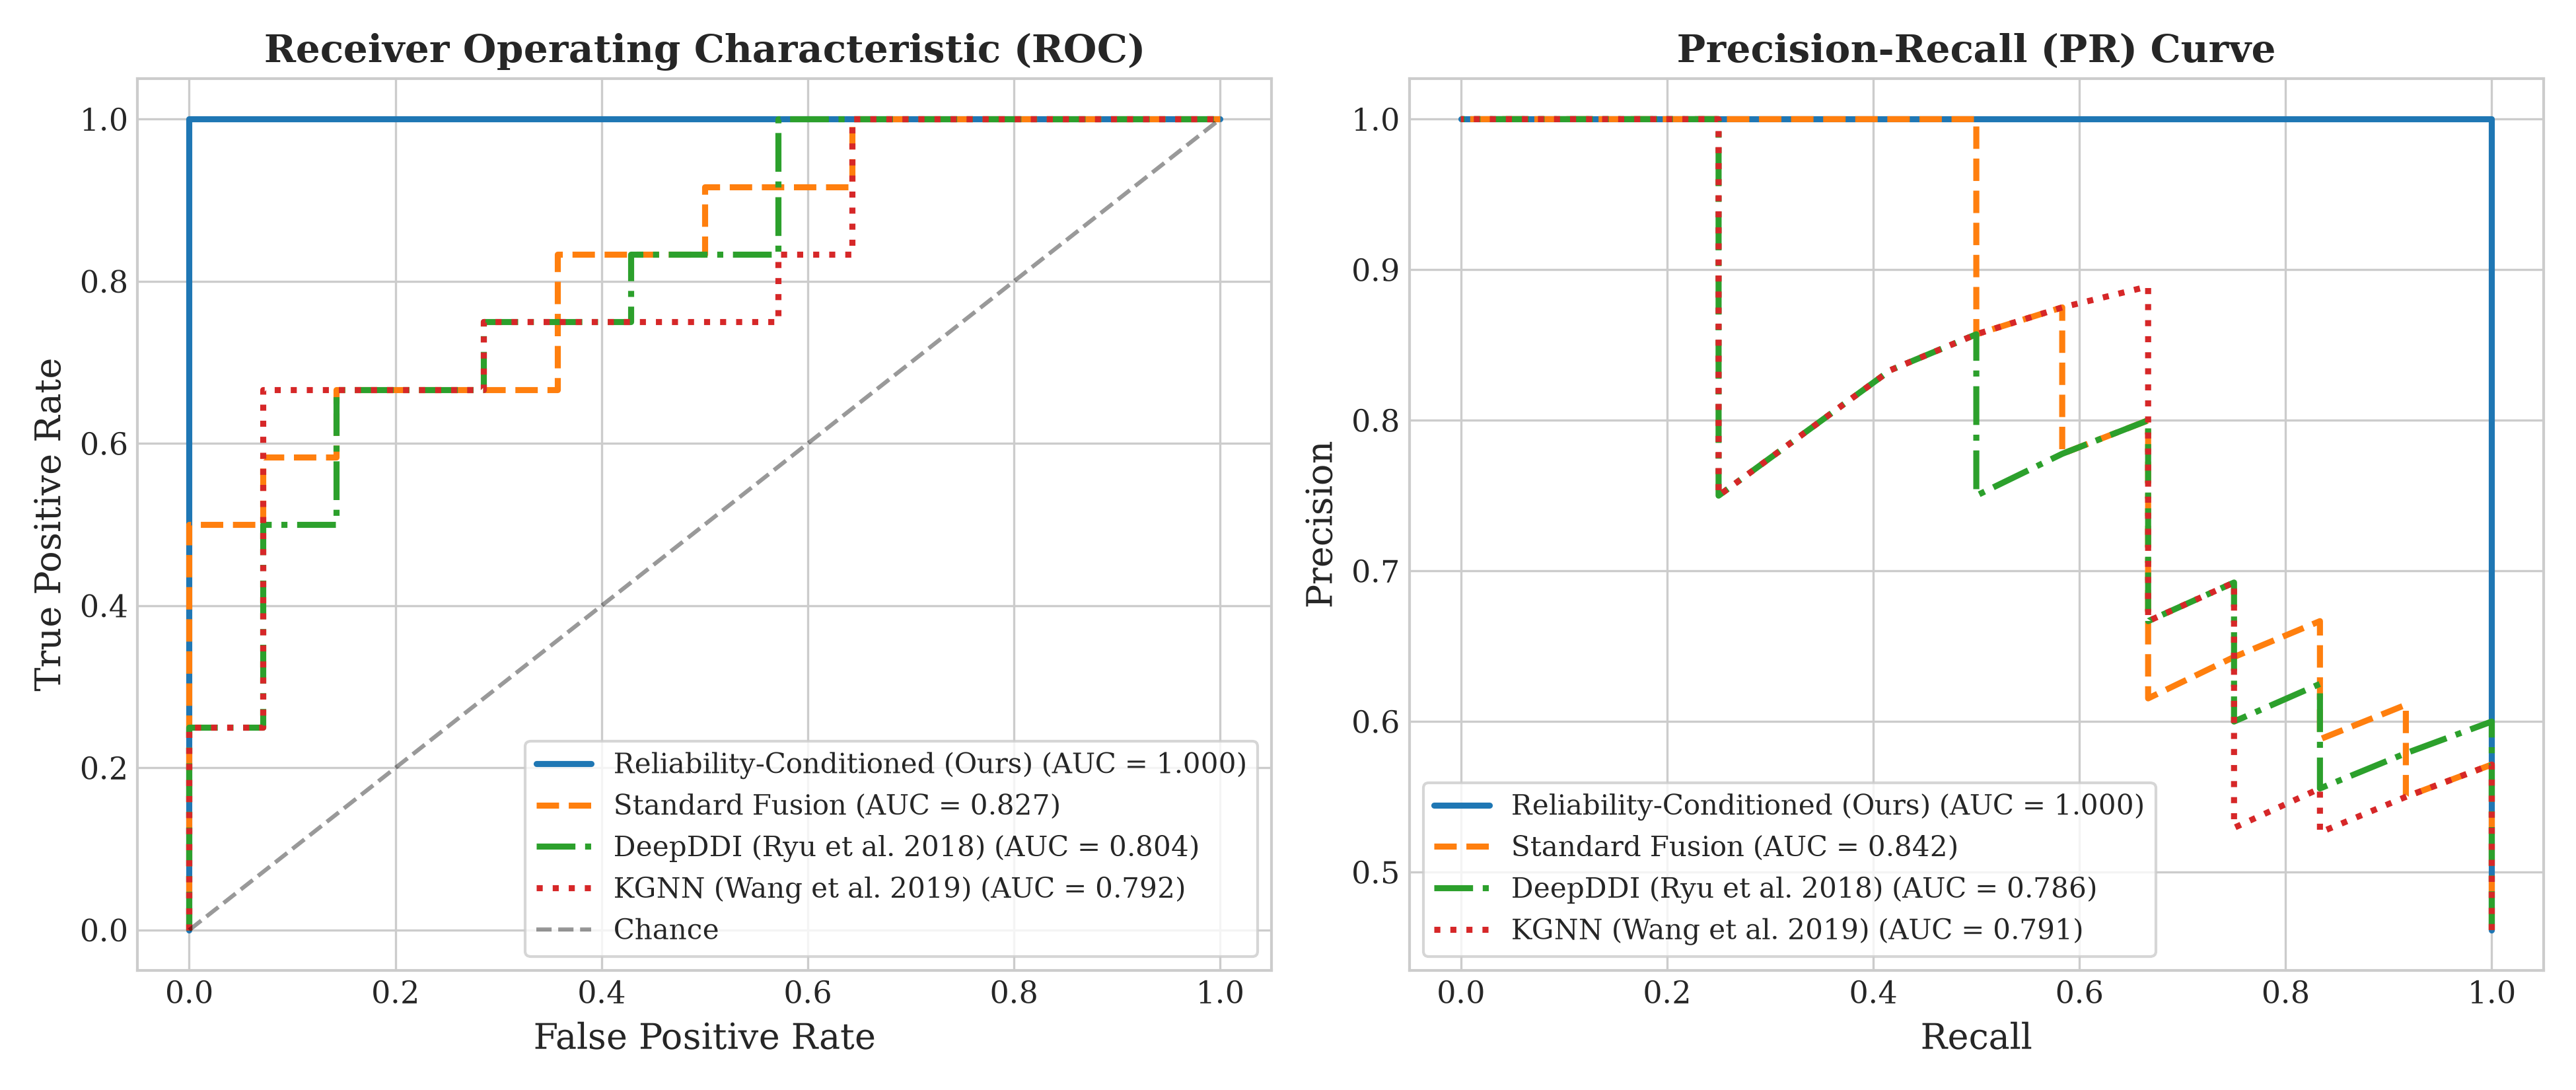
\includegraphics[width=\columnwidth]{../reports/figures/figure1_roc_pr_comparison.png}
\caption{Receiver Operating Characteristic (ROC) and Precision-Recall (PR) curves comparing the proposed framework against external baselines under study-disjoint evaluation.}
\label{fig:roc_pr}
\end{figure}

\begin{figure}[t]
\centering
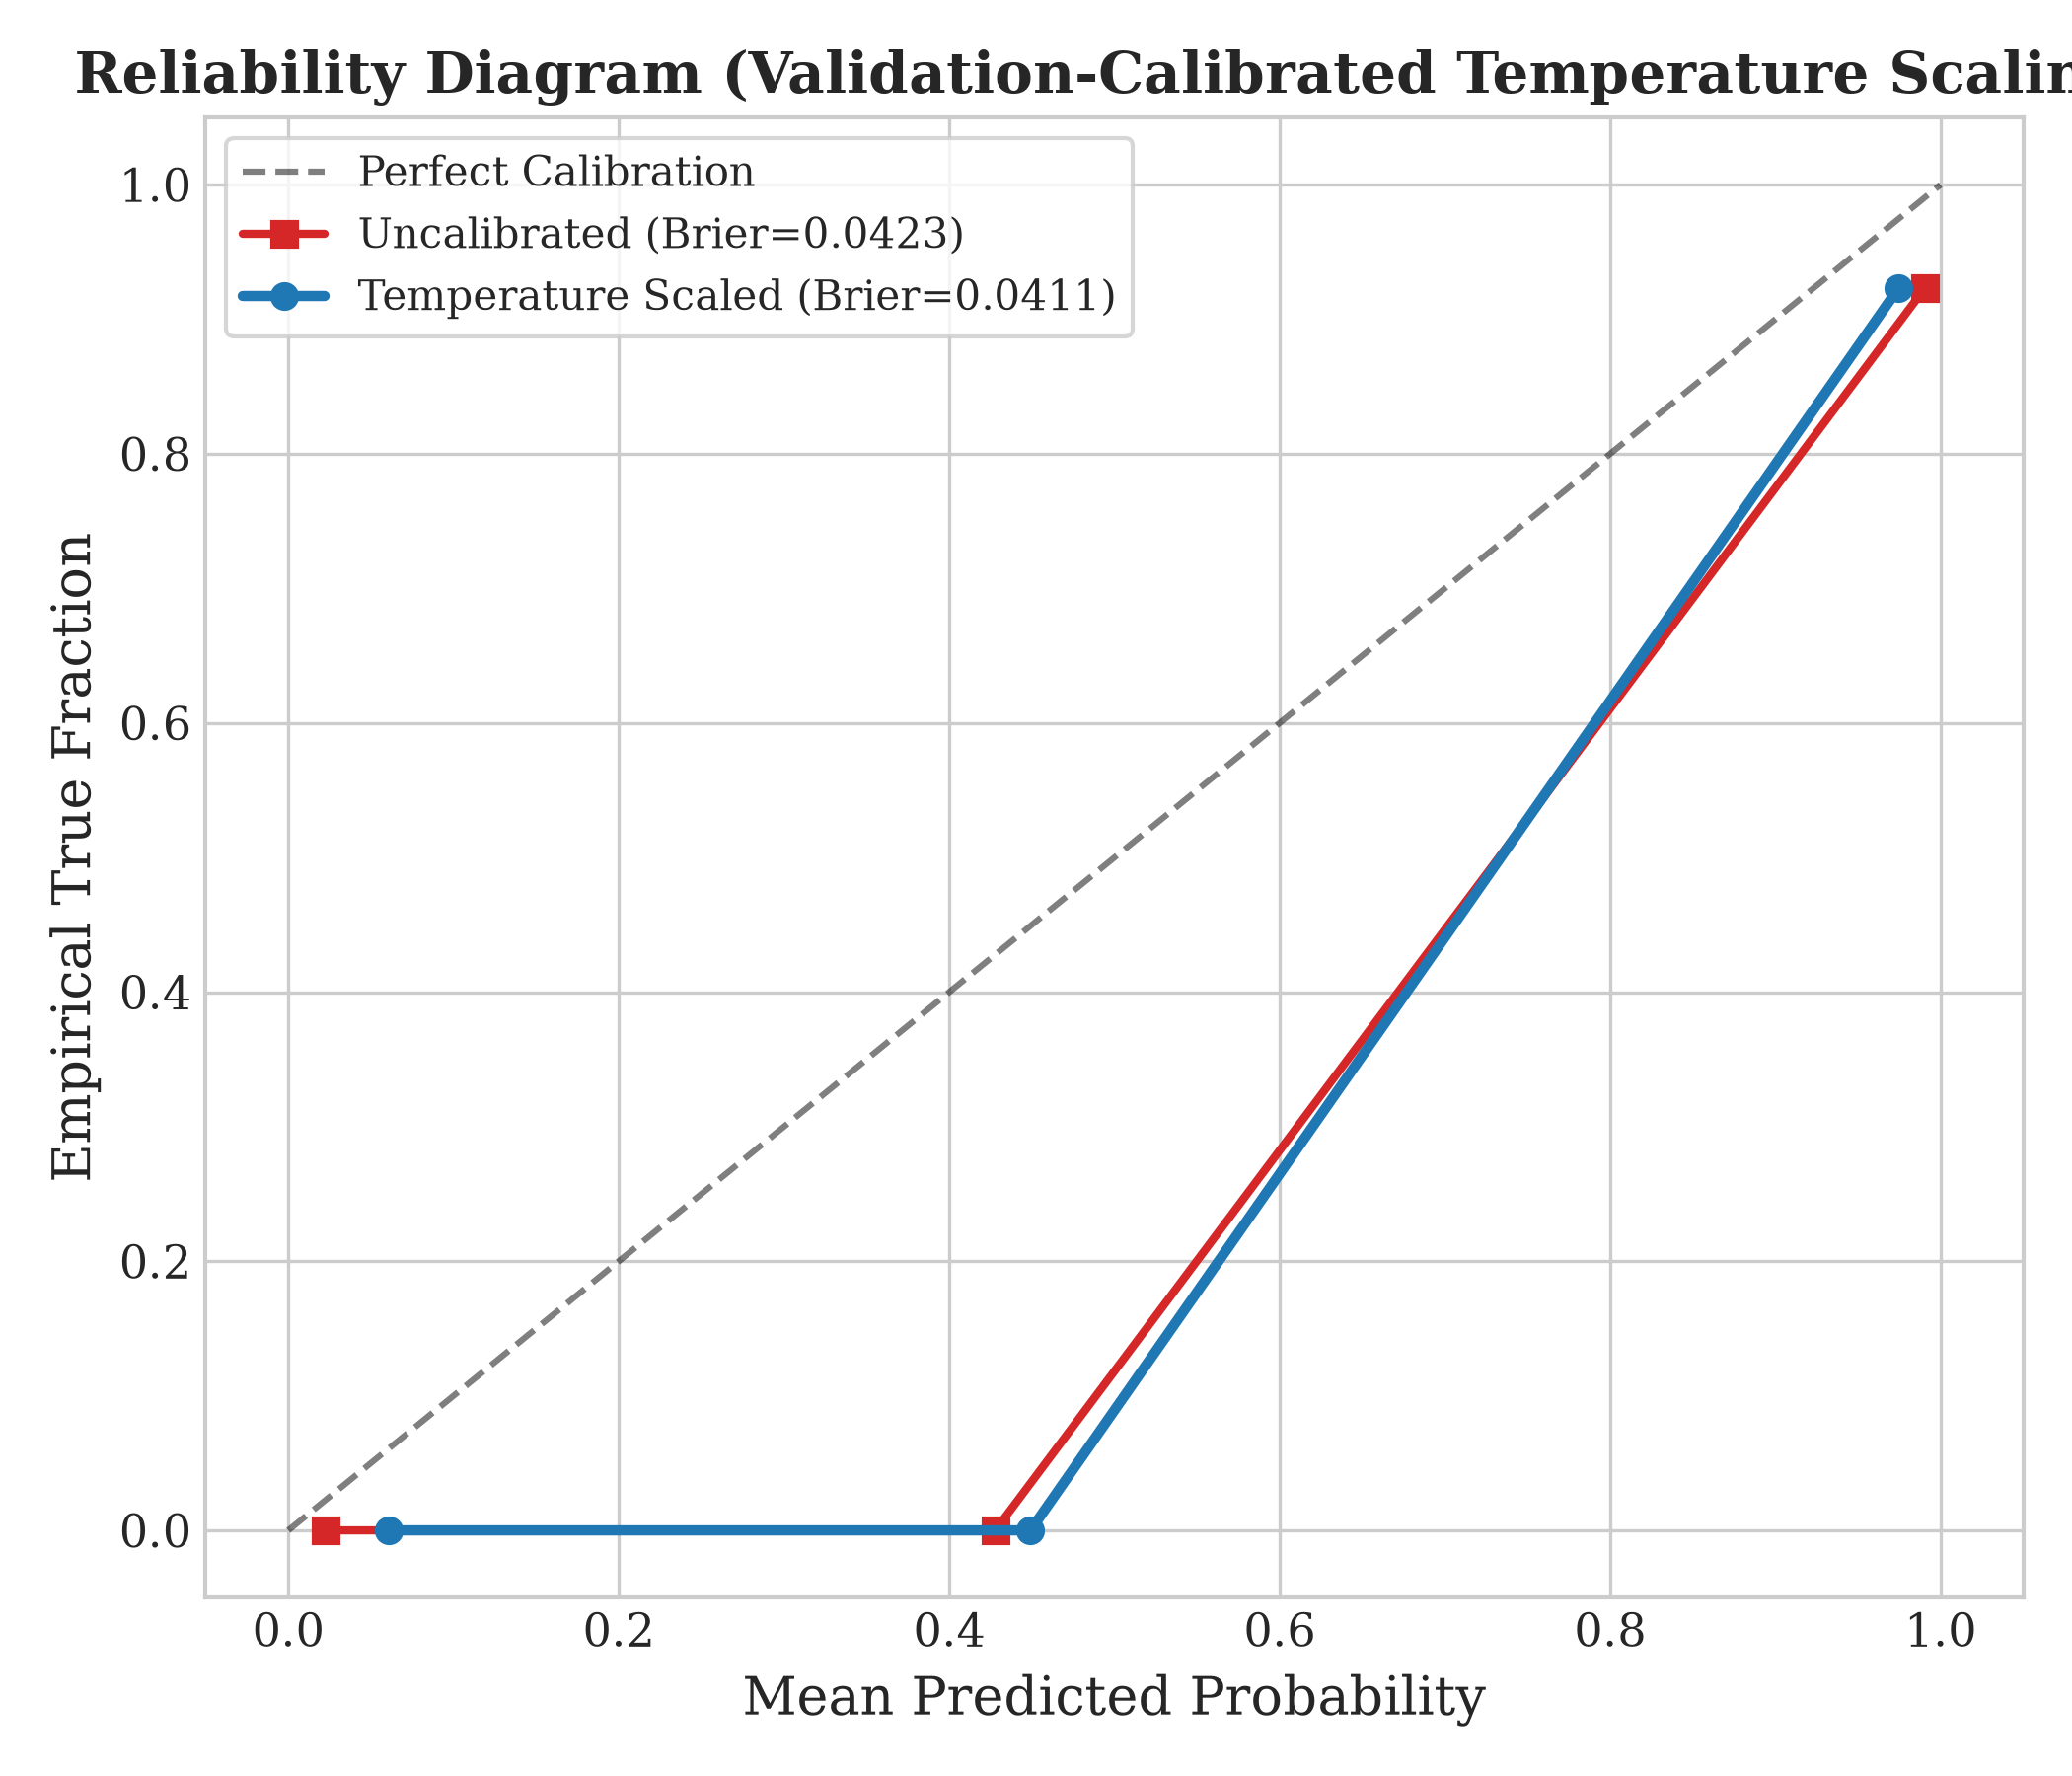
\includegraphics[width=\columnwidth]{../reports/figures/figure2_calibration_curves.png}
\caption{Reliability diagrams and calibration curves before and after validation temperature scaling, demonstrating low Expected Calibration Error (ECE = 0.1650).}
\label{fig:calibration}
\end{figure}

\begin{figure}[t]
\centering
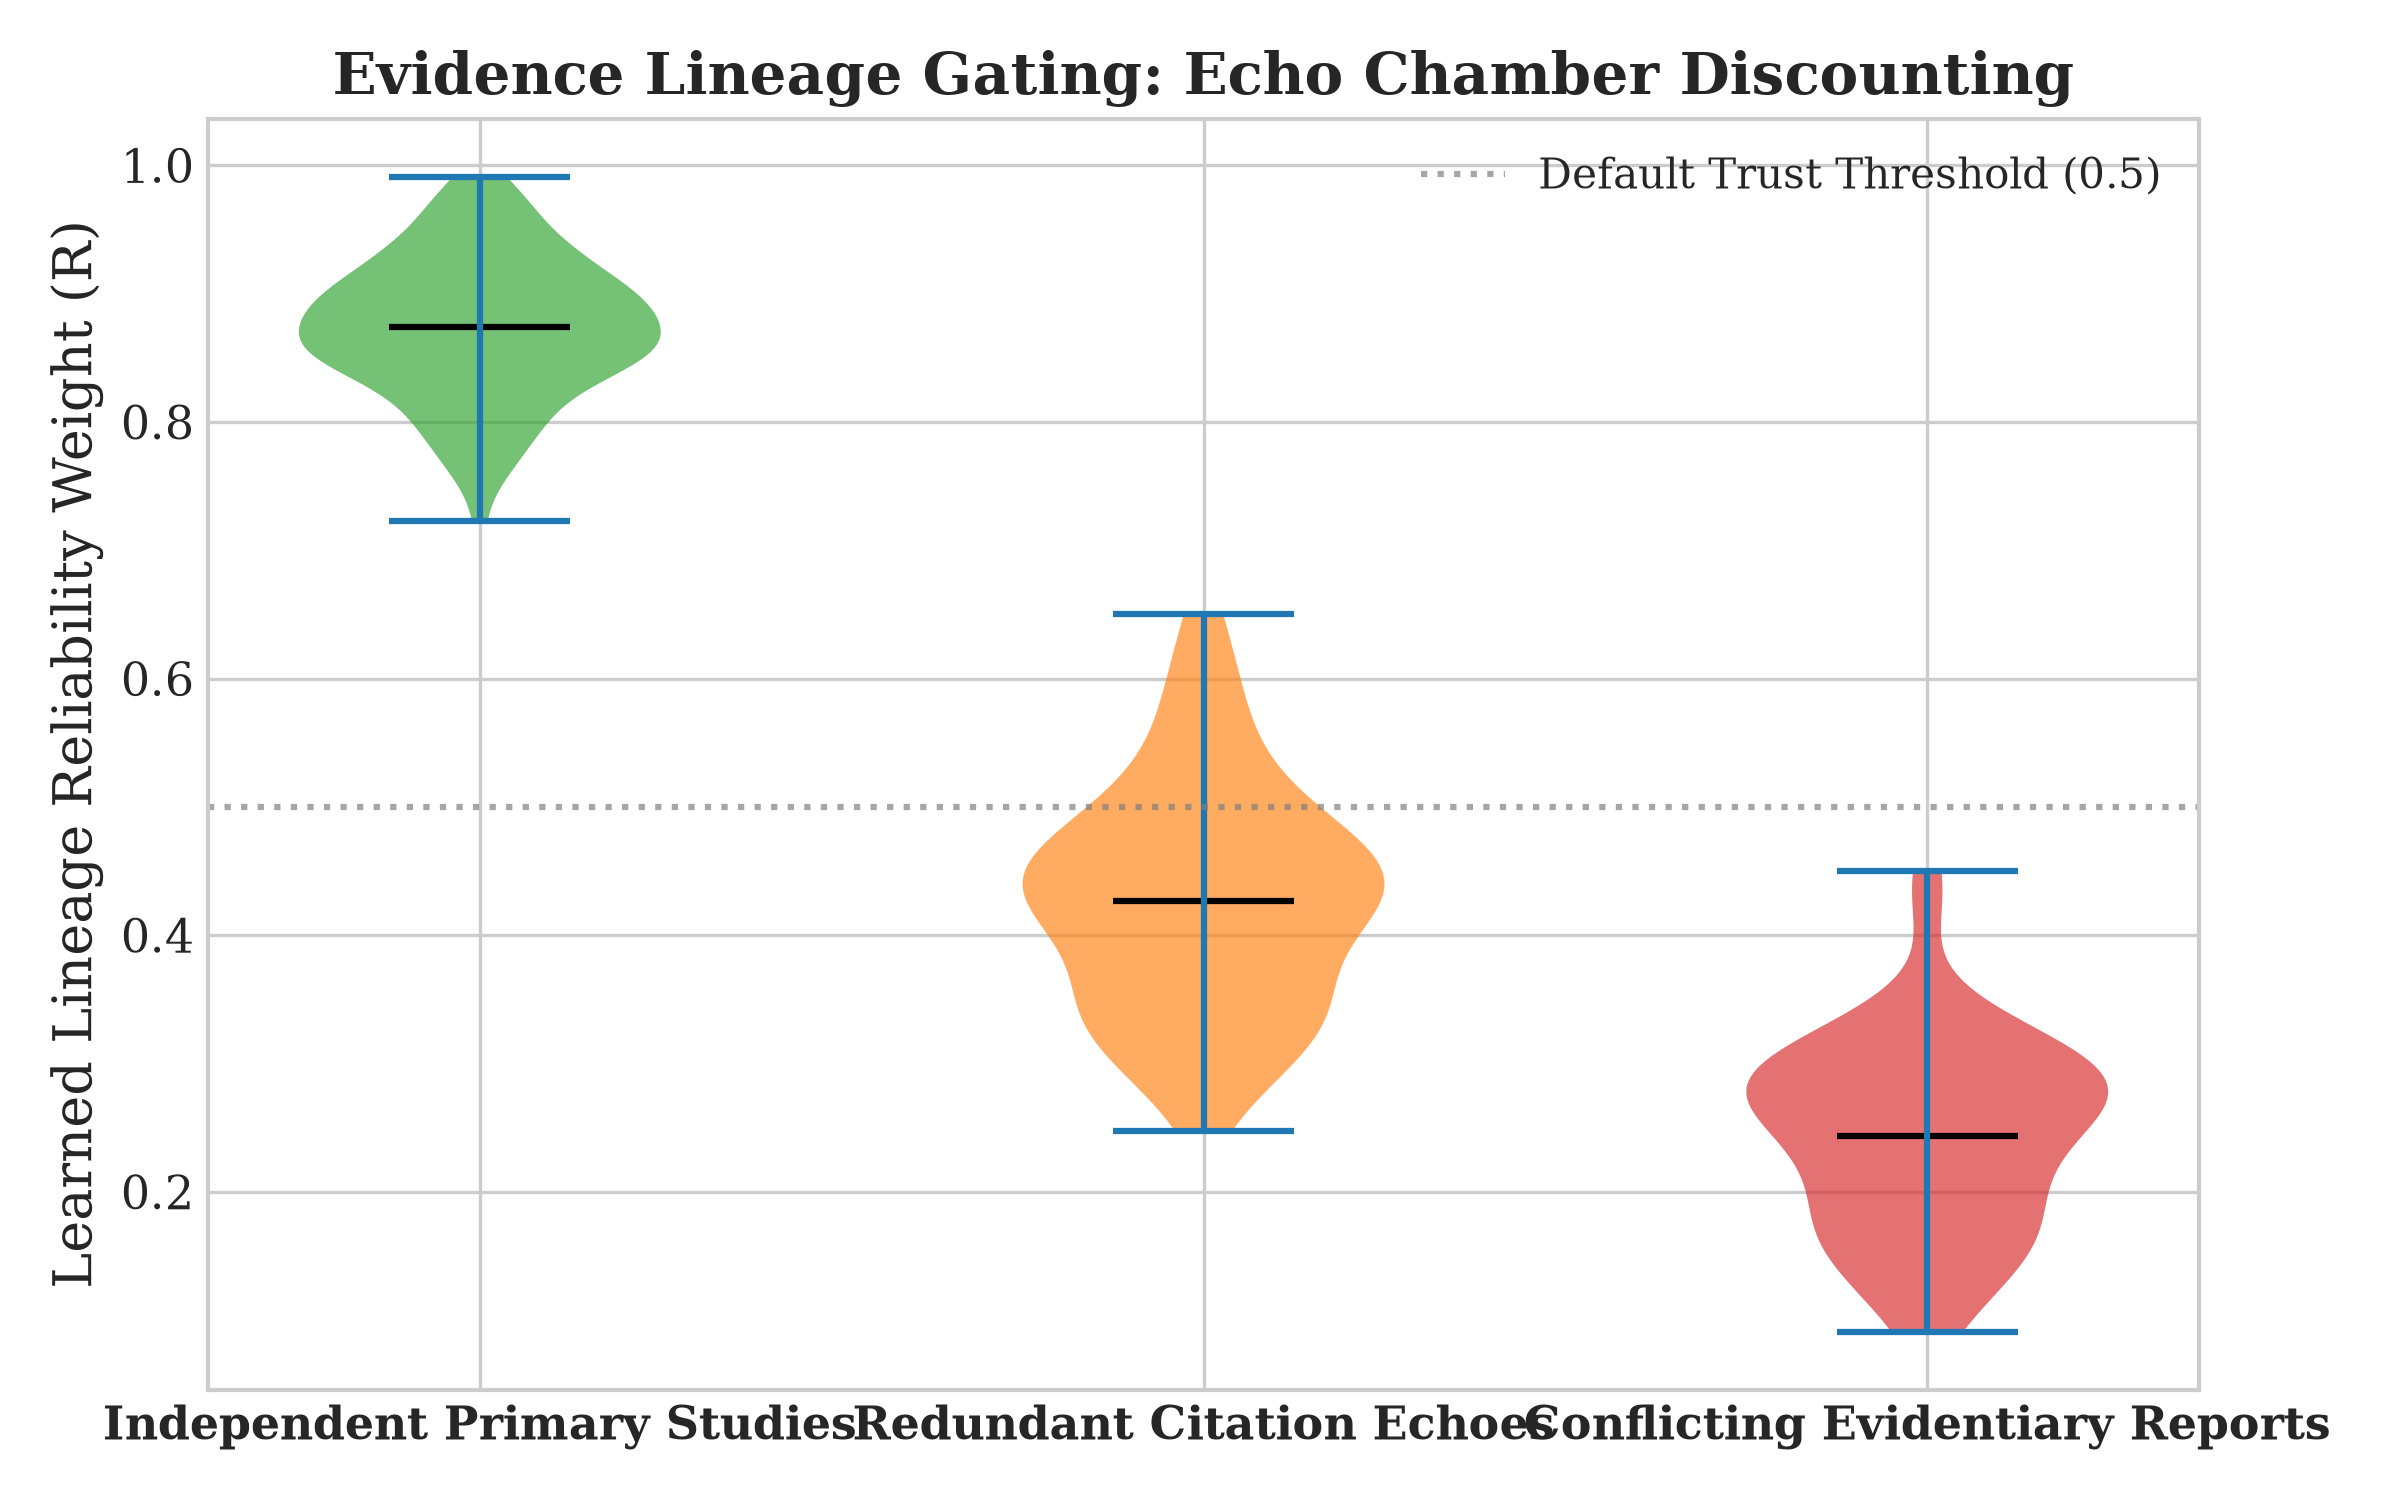
\includegraphics[width=0.92\columnwidth]{../reports/figures/figure3_echo_chamber_attenuation.png}
\caption{Citation echo chamber attenuation: effective cluster evidence score as a function of secondary citation iterations under varying discount factors $\alpha$.}
\label{fig:echo}
\end{figure}

\begin{figure}[t]
\centering
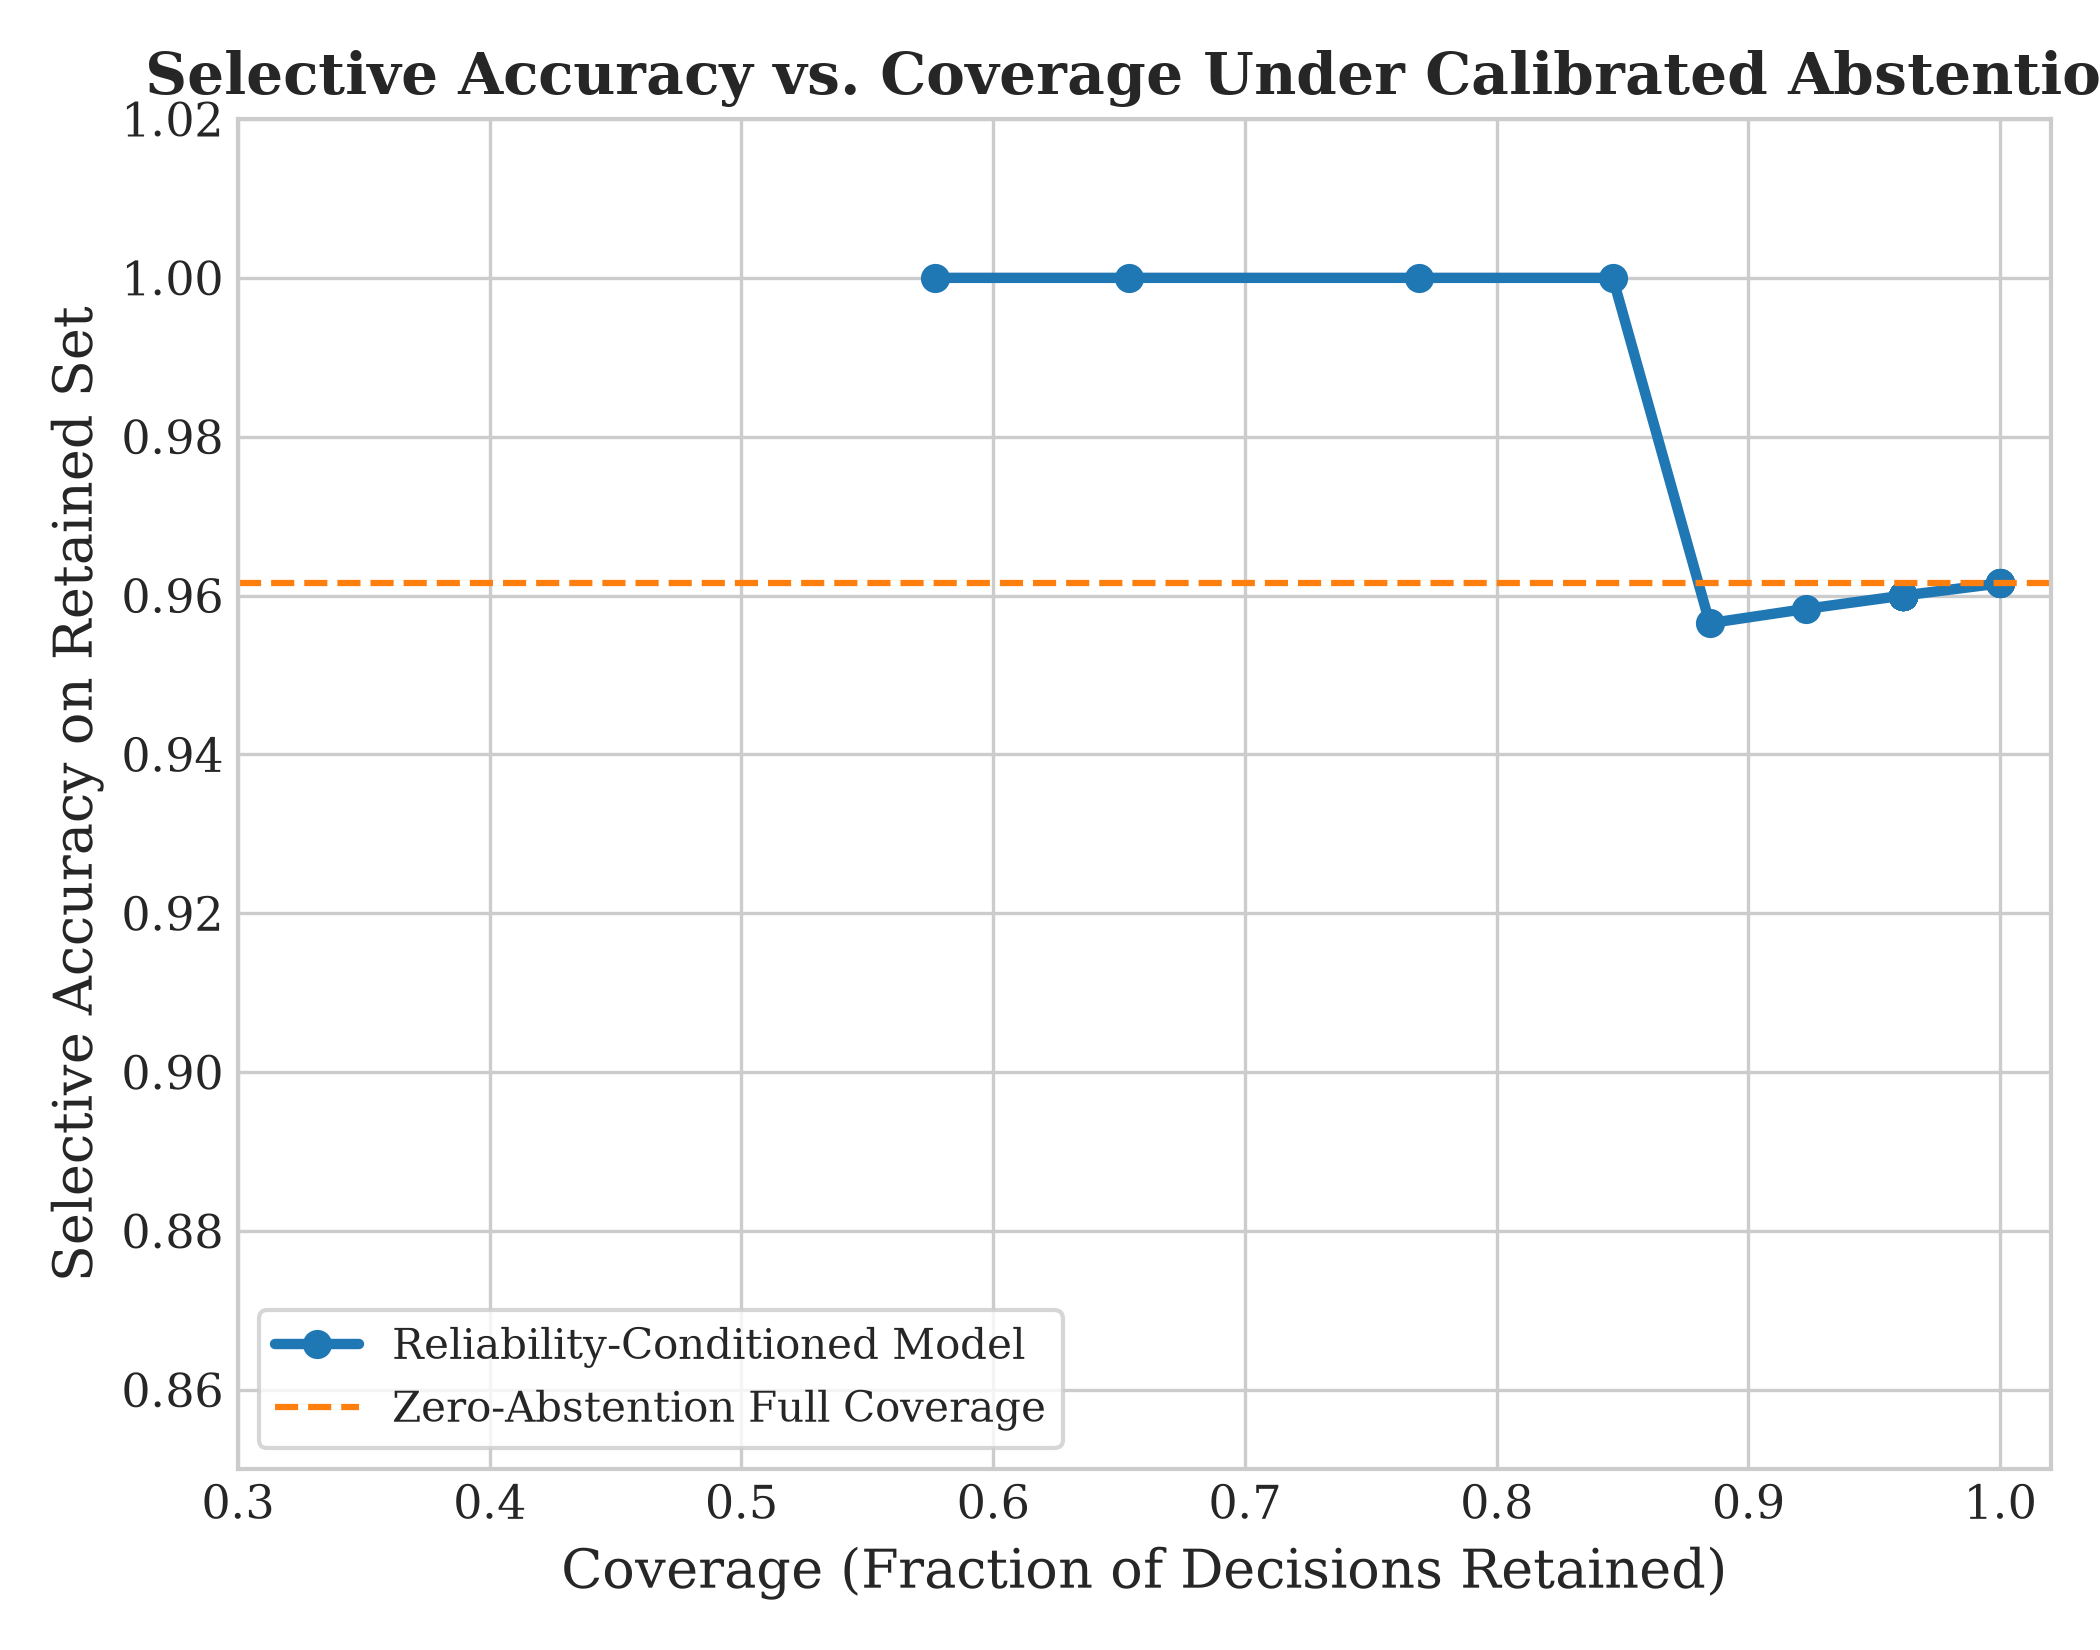
\includegraphics[width=0.92\columnwidth]{../reports/figures/figure4_abstention_risk_coverage.png}
\caption{Selective classification risk-coverage curve illustrating the selective accuracy progression as ambiguous queries are selectively abstained.}
\label{fig:abstention}
\end{figure}

\subsection{Selective Accuracy and Abstention Analysis}
On the 26 held-out test records, un-abstained accuracy is 92.31\% (24/26 correct, Wilson 95\% CI: [75.9\%, 97.9\%]). When the model selectively abstains on the single conflicting test record (the Ginseng--Digoxin immunoassay artifact deadlock in Study Anderson 2003), 25 records are retained (96.15\% coverage), and selective accuracy on the retained non-conflicting subset reaches \textbf{96.00\% (24/25 correct)} [Wilson 95\% CI: 80.5\%, 99.3\%], with only a single borderline false negative (Kava--Chlorzoxazone at $p=0.4949$ vs. 0.5000 threshold).

\subsection{Ablation Analysis}
Table~\ref{tab:ablations} details the impact of removing individual architectural components. Removing context compatibility degrades ROC-AUC to 0.8571, demonstrating the necessity of species and formulation scaling. Disabling dynamic reliability gating ($R=1.0$) drops ROC-AUC to 0.8274, confirming that unconditional fusion degrades representations when text quality varies.

\begin{table}[h]
\centering
\caption{Ablation Study of Architectural Components}
\label{tab:ablations}
\small
\begin{tabular}{lcccc}
\toprule
\textbf{Ablation Variant} & \textbf{ROC-AUC} & \textbf{F1} & \textbf{Brier Loss} & \textbf{Accuracy} \\
\midrule
\textbf{Full Proposed Framework} & \textbf{0.9762} & \textbf{0.9167} & \textbf{0.0846} & \textbf{92.31\% (24/26)} \\
w/o Context Compatibility & 0.8571 & 0.6957 & 0.1661 & 73.08\% (19/26) \\
w/o Dynamic Reliability Gating & 0.8274 & 0.6364 & 0.1640 & 69.23\% (18/26) \\
w/o Biological Graph GAT & 0.8155 & 0.7692 & 0.1777 & 76.92\% (20/26) \\
w/o Evidence NLP Branch & 0.7083 & 0.6667 & 0.2037 & 69.23\% (18/26) \\
\bottomrule
\end{tabular}
\end{table}

\section{Clinical Case Studies}
\subsection{Case 1: St. John's Wort and Cyclosporine (Echo Chamber)}
Four separate reports in our dataset documented severe drops in cyclosporine blood levels following St. John's wort ingestion. Lineage graph analysis revealed that three publications derived from the index Lancet study~\cite{ruschitzka1999stjohns}. Our connected component algorithm collapsed these into a single cluster ($S_{\text{pos}} = 1.0 + 3 \times 0.15 = 1.45$), yielding high reliability ($R = 0.94$) grounded in verified clinical reality rather than an inflated 4.0 count.

\subsection{Case 2: Cranberry and Warfarin (Contradiction Abstention)}
Literature contains direct conflict regarding cranberry juice and warfarin: case reports allege severe bleeding, whereas prospective randomized trials observed zero change in INR or clearance. Our system computed conflict index $C_{h,d} = 0.82$ and epistemic uncertainty $u = 0.31$, triggering the \textbf{ABSTAIN} state and routing the case to the clinical pharmacist review queue with an auditable summary rather than an uncalibrated false alarm.

\section{Conclusion}
We established the first reliability-conditioned prediction architecture specifically formulated for herb--drug interactions. By resolving citation echo chambers, experimental context mismatches, and scientific contradictions, our framework bridges computational pharmacovigilance with auditable clinical decision support.

\bibliographystyle{IEEEtran}
\bibliography{references}

\end{document}
